
\chapter{\label{ch:3-design} Design and Implementation}

%\minitoc


\section{Aims and Objectives}
\subsection{Aims}

The primary aim of this project is to explore methods for text generation and then develop a system through which prose about movies can be generated. This prose should be in the form of a movie review, and should pick the most recurrent points or themes in a corpus of movie reviews discussing a singular movie.

\subsection{Objectives}
To explore methods for generating text which reviews film.
To develop a natural language generation system which picks points from multiple review texts and uses them to structure an informed review.\\
To develop an online platform to host generated movie reviews which can gather feedback and data on the reception of said review.\\
To develop an autonomous bot that can discuss movies (or at least reply with an opinion of a movie) over twitter. Ideally this would drive traffic towards the movie review blog which hosts reviews made by the bot.

\section{The Structure and Content of a Movie Review}
From reading movie reviews from various sources and types of publication (such as user-submitted reviews as well as articles in publications or on their websites) attempting to observe their structure, I have found that between different movie reviews the structure typically varies wildly and different reviews focus on many different aspects of a film. Depending on the movie and the reviewer, many different topics can be addressed.
Typically, more comprehensive reviews such as those published on news websites include an introduction touching upon the more important or noteworthy details of a film, followed by brief plot synopsis which may or may not be used as a vessel for the review of each element of the film as it becomes relevant within the context of the plot synopsis. 
After this, reviews typically get more in to detail on the film, commenting on how the cast and crew have performed, noteworthy themes and topics and other evaluative sentiment.
To close the articles, they usually make a recommendation of the film, or some kind of statement about its quality. \\
User submitted reviews typically are shorter, and tend to focus more on elements a user particularly enjoyed, or quite often disliked (I have found user reviews tend to skew towards either glowing or completely negative with usually less cases for a middle ground). These usually focus on the believability of performances, special effects and other things that are much more immediately obvious than some of the topics paid reviewers address.\\
This, while general, gives me something to work with in terms of determining the kind of content that should go into a generated movie review.\\



\section{Planned Order of System Development}
Three methods of generating prose are planned. The first, utilising Markov Chains and input of specific movie reviews or tweets. The second, a template-driven system which will require movie metadata as well as a corpus of text on which to perform sentiment analysis.
The final, an NLG system which will require further metadata as well as the corpus of text obtained from the template driven system in order to generate a review.\\

I planned to implement the Markov chain system first, since it required the least data and its relative ease of implementation. Data is to be obtained through twitter search or from a movie review as an input. The second system to be the template system, as it required the second least input data, and this data gathering can be iterated upon in the NLG system, which is why I chose to implement this last.\\

As well as this, it is planned that a twitter bot, and blog website be implemented in order to collect data on these systems working in the real world. These are planned to be implemented in tandem with these other systems - the Twitter bot needing to be made live after or at the same time as the blog is developed, as its main purpose is to drive traffic towards the reviews generated.\\
\begin{figure}
\centering
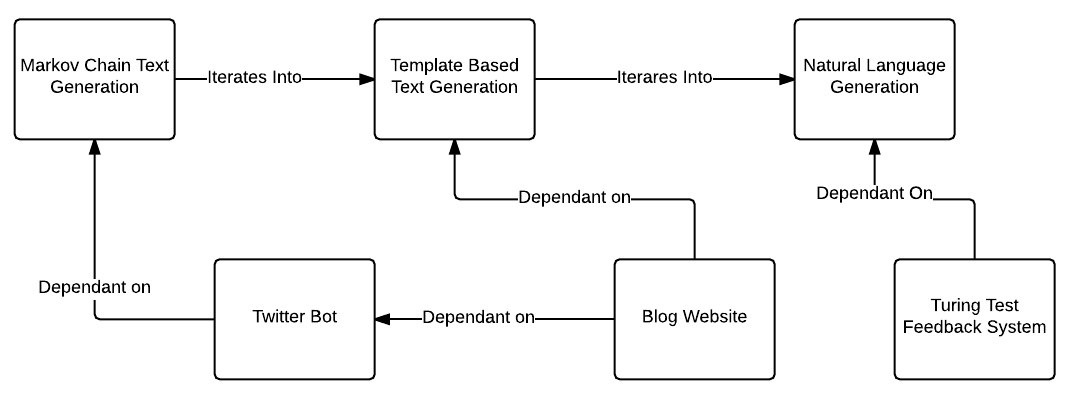
\includegraphics[width=0.7\linewidth]{figures/diagrams_etc/system_iterations}
\caption{Proposed order of development for systems. Dependencies indicate works that be used without the other but does not require the system to be implemented}
\label{fig:systemiterations}
\end{figure}

\section{Markov Chain for Text Generation}
Markov models represent a series of possible events whose occurrences depend only on the last event which happened. The probability of each event occurring is based on how frequently this event occurred in the data it is given. For example, a Tuesday would have a 100\% chance of transitioning into a Wednesday, given an input sequence of a week.\\
When representing language, these models are built from input corpora, and take a number of n-prefix words to model a point in the chain, and the list of single words (as well as their occurrences) preceding them in the corpus to represent the potential outputs. For example, the sentence "the dog and the hound the cat and the walrus" would produce a chain (with 2 preceding words) in the form of:


\begin{center}
	\begin{tabular}{ |c|c| } 
		\hline
		the dog & and \\ 
		dog and & the\\ 
		and the & hound, walrus\\ 
		the hound & the\\
		hound the & cat\\
		the cat & and\\
		cat and & the \\
		the walrus & (no value)\\
		\hline
	\end{tabular}
\end{center}

This kind of table could then be used to produce an output of text by selecting a starting point, stochastically or arbitrarily (such as at the beginning), and following the chain, choosing its next word based on the occurrence of the preceding word.
It could generate "the dog and the walrus" or "the dog and the hound the cat and the hound the cat and the hound the cat and the walrus". The chain could repeat "the hound the cat and the hound..." indefinitely if other ending conditions were not specified, such as a word or character count.\\

My implementation includes a breaking point of a character limit, as well as taking multiple documents (as opposed to a single long text) to build a chain in order to accommodate for using data sources such as twitter in place of longer texts, depending on what is being generated.\\

\begin{figure}
\centering
\includegraphics[width=0.7\linewidth]{"figures/diagrams_etc/MarkovChain-GenerateTable - Page 1"}
\caption{Flow chart demonstrating the construction of a Markov model for text input}
\label{fig:markovchain-generatetable---page-1}
\end{figure}


\begin{figure}
\centering
\includegraphics[width=0.7\linewidth]{"figures/diagrams_etc/markov_generatetext - Page 1"}
\caption{Flow chart demonstrating how text can be generated out of a Markov model}
\label{fig:markovgeneratetext---page-1}
\end{figure}



\section{Template-Based System for Text Generation}
The design of this system started with the premise of filling out template sentences for segments of a review in a random fashion until a text of a satisfactory size is produced. The initial idea being that an introduction is filled in, then a brief plot synopsis, some text evaluating the performances of actors and noteworthy crew (such as the director or writers) and then a closing statement regarding whether or not its worth seeing a film.\\

The first step of the template system is data gathering.

It web scrapes a corpus of movie reviews for a given movie from IMdB. These are user reviews taken from a movie's reviews page, and an amount are taken sorted by their highest rating. Then it web scrapes plot synopsis, also from IMdB this is then summarized using the TextRank algorithm. It finally uses themoviedb's API to gather metadata about a film, which in this case is the cast and crew, their roles, and the genre.\\


The second step in this process is then forming an understanding of that data.
First is the separation each review text into a large list of sentences so that they can be tagged and analyzed for sentiment.
Categorise each sentence as about a particular topic or person (cast, crew, director), using the metadata gathered from the OMDb (the Open Movie Database) API to match sentences to these topics. Sentiment on each member of cast and crew as well as the director is then evaluated by the total value of these sentiments (a sentiment tagged sentence has a positive, negative and neutral value, and I measured polarity based on the larger of the two sums of positive or negative values).\\

The rest of the process is then building a review text out of templated sentences until completion.
First, a templated introduction is selected and then filled out. This is a sentence that has missing sections to be filled in with factors such as the director, the name of the film, actors and their roles, and sentiment based adjectives and adverbs. In the templates, they are indicated by being surrounded by square brackets, such as '[director]', or '[genre]' - indicating they need to be filled by the name of the director and the name of the genre.\\ 
For the introduction, the aim was to inform the reader of the film's name, the director, some general sentiment, and the name of at least one actor and their role. Next, the TextRank summarized plot summary is inserted into the document, then it goes through several rounds of filling randomly selected templates to create a main body of review text, much in the same way as the introduction. The content of the main body consisted of evaluation of members of the crew, cast and director, providing adjectives and adverbs to add the illusion of informed opinion and sentiment. Finally an outro template is selected and then filled. \\
The outro template consists of a sentence that recommends the movie based on some factor such as the performance of the director, an actor, general sentiment and liking the genre. It too uses the Part of Speech tagging method, or a general sentiment based word selection.\\
Adjectives and adverbs in this review were selected in one of two ways, depending on the parameter given to the system. The first was a simple polarity based selection of 'good' or 'bad', 'well' or 'poorly' that fill out the templates appropriately, although in a fairly bland style. The second used a Part-of-Speech tagging system to retain all of the adjectives and adverbs from the sentences related to the subject we wish to add sentiment to, and then these words individually tagged using the VADER sentiment analysis method included in NLTK to return a (hopefully representative) sentiment. In the absence of any adjectives or adverbs in the corpus, the simple polarity words are returned.

\begin{figure}
\centering
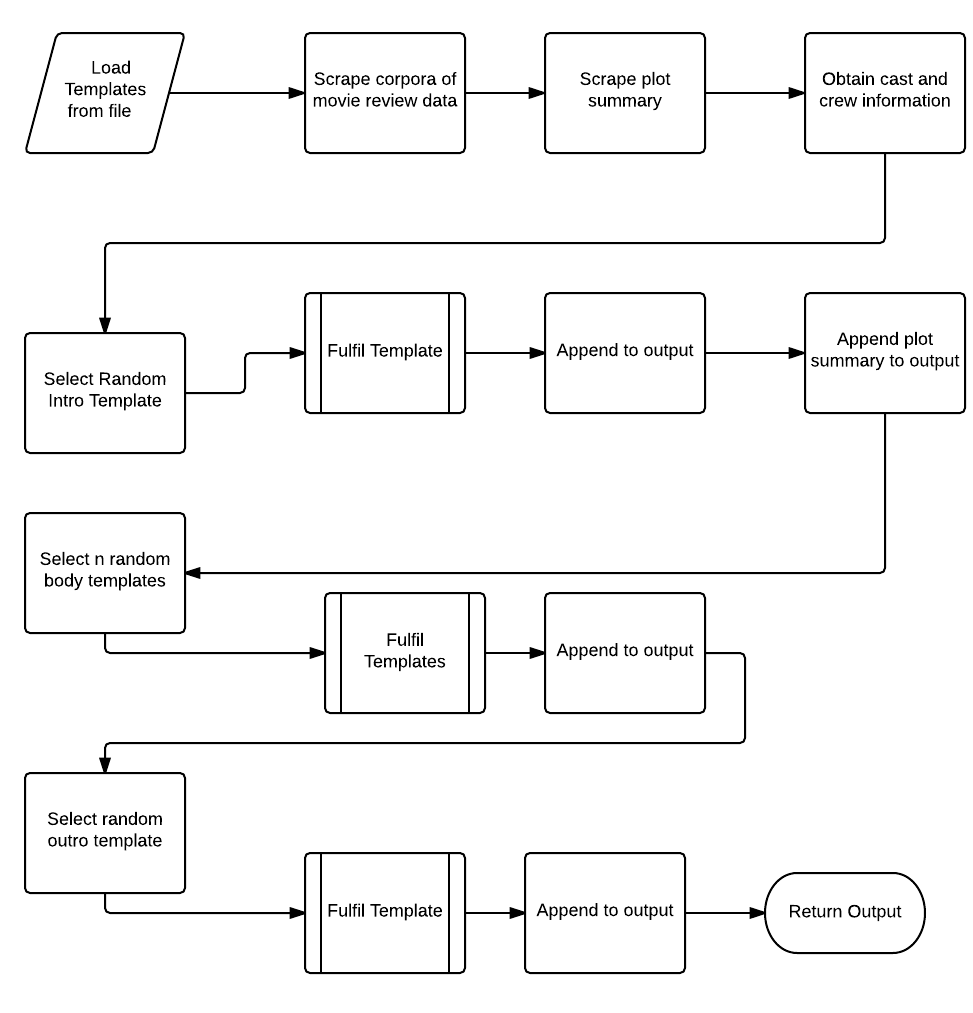
\includegraphics[width=0.7\linewidth]{figures/diagrams_etc/template_system}
\caption{Flow chart visualising the process of the template-based system.}
\label{fig:templatesystem}
\end{figure}


\section{NLG System}
The design of the NLG system is in line with the 6 phases outlined by Dale and Reiter in 'Building Natural Language Generation Systems', although it was difficult to design a system which could report opinion.
\begin{figure}
\centering
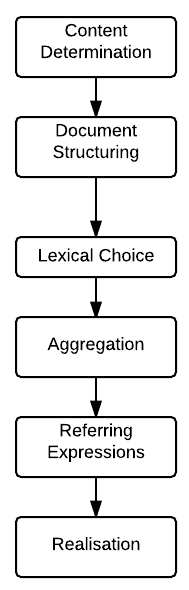
\includegraphics[width=0.7\linewidth]{figures/diagrams_etc/nlg_toplevel}
\caption{Visualisation of the top-level processes for a NLG system.}
\label{fig:nlgtoplevel}
\end{figure}

Content determination:\\
Content determination is the step in the process which simply involves deciding what content should be included in the generated document.
It proved difficult to gather all of the right content that is commonly discussed within the domain of a movie review. I limited the range of discussion to the cast, crew, director and their performances, as I did not have time to develop a method for discovering the presence of the discussion of abstract topics such as tone or themes in text.\\

For my purposes this stage involves data gathering and web-scraping, as well as making decisions as to what of this data is used in the document. 
Much like in the template-based system, the first step is obtaining all of the data I need for generating a document. I reuse all of the data-gathering methods from this system, but while I am forming an understanding of this data, I also search for the past appearances of the most relevant cast and crew in other movies, as this provides more content to discuss. This uses the TMDb 'Discovery' API, which did require some working around as multiple names in a search would not return films that only included the given cast and crew names.\\

As mentioned previously, some determination of the most relevant members of the crew is made. It seemed most intuitive to design this as a simple search for the n-most frequently mentioned members of the cast and crew to put into the film review. Arbitrarily I chose 4 members of the cast, and 3 members of the crew as maximums, and iterated through the list of sentiment-tagged sentences associated with each member of the cast and crew.\\

With all of this data attained, the content determined is surmised as a list of the most important cast members with all the sentiment tagged sentences which mentioned them, with the same for the crew, and the director. Of course the title of the film is also a part of the content determined, as well as the genre, and a general overall sentiment to help decide on a tone. These elements have been gathered in the same way as they have in the template based system. I did choose to drop the plot synopsis, as I felt it did not provide particularly brilliant shortened forms from the use of TextRank, and copying a plot synopsis verbatim in order to seem more human felt inappropriate as it is a piece of writing that has actually been created by a human and not modified at all.\\

\begin{figure}
\centering
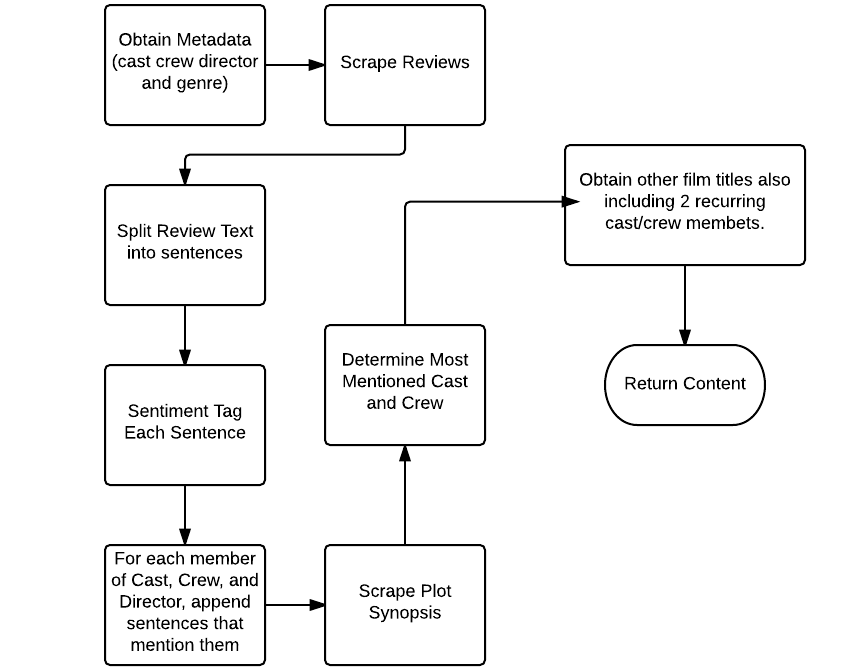
\includegraphics[width=0.7\linewidth]{figures/diagrams_etc/content_det}
\caption{Demonstration of the content determination process}
\label{fig:contentdet}
\end{figure}


Document Structuring:\\
This is the stage which involves deciding the order of the document. For my generation of a movie review, I decided that this stage involved the structuring of an introduction, main body of evaluative text, and an outro consisting of a closing statement and recommendation of the film.
I decided that this structure should be built upon the inclusion of specific clauses, which could later be aggregated into full sentences and pieces of content.\\

The structure of the document is stored as a list of clauses, along with the relevant data that should be used to fulfil that clause.\\
The introduction and ending statement of the review is structured in a different manner to the main body, which is simply the random selection of relevant topics to include inside of an introduction and outro, and placing each of these topics into a clause alongside the data that fulfils it.
Topics included in the introduction are mention of the film's title, the films genre, the director (optionally including how well he performed), an overall sentiment of the film, and mention of the most relevant actor and his role (as well as the second most relevant actor, randomly).
The 'outro' handles its structure in the same way as the intro, choosing from the topics of overall sentiment, the most relevant actor, the director, and the genre. It is worth noting that these structures may appear to be very similar, although the clauses are specified to be part of an outro or intro which is intended to change how they are worded.\\

The main body of the document is somewhat structured in a similar manner, although repetitions of the type of clause are made, rather than being limited to one mention at the most in the case of mentioning different members of the cast or crew. The topics to choose from were decided to be an assessment of the director, assessment of the cast and crew as well as mentioning their roles, additionally whether or not the actors were better or worse in past roles that they had worked together in (such as Quentin Tarantino and Samuel L. Jacksons performances being compared between Pulp Fiction and Jackie Brown). If past work had been found, other clauses concerning people involved in this past work were mentioned close to this comparison.\\
After this, the rest of the cast, crew and director if still not mentioned in evaluation are then given clause pairs concerning their performance and describing their roles.\\
When cast or crew members are mentioned, they are done so with pairs of clauses - one of which gives sentiment and another which describes their role or job. The order of the clauses is random and intended to make the description of the same type of thing multiple times seem more human in its variety.\\

\begin{figure}
\centering
\includegraphics[width=0.7\linewidth]{"figures/diagrams_etc/structure document"}
\caption{Diagram of the general document structuring process}
\label{fig:structure-document}
\end{figure}


Aggregation:\\
This stage involves combing the document structure in order to combine clauses into sentences so that they are more readable and flow more effectively. For example, the combination of two clauses such as "Actor plays the role of Character" and "Actor was believable" being aggregated into "Actor plays the role of Character believably", or "Actor was believable in the role of Character" depending on the order these clauses were determined to be placed in.\\
The introductory clause is concatenated into a single sentence concerning all of the topics it hits upon, maintaining the order each item is mentioned. The outro is also handled like this in order to make it more simple to handle during lexical choice, although it is not necessarily intended to be a single sentence.\\

\begin{figure}
\centering
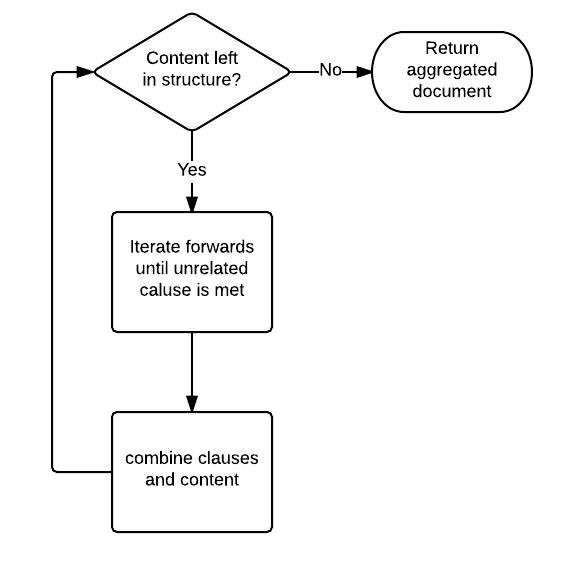
\includegraphics[width=0.7\linewidth]{figures/diagrams_etc/aggregateDocument}
\caption{Simplified visualisation of document aggregation.}
\label{fig:aggregatedocument}
\end{figure}

Lexical Choice:\\
The choice of how exactly to word each of these sentences was quite a difficult problem to solve. I initially wanted to model the language in subject-verb-object pattern objects but realised that it would be more efficient to fill in patterns that already matched these sentences with pre-determined lexical choices, save for sentiment related adverbs and adjectives which would be chosen from the collection of sentences associated with the topic lexical choice was being made for. It also became clear that this was generating quite bland sentences, even with differing wording, so I included the insertion of sentiment based templates to add further variety to the text.\\
In order to make these lexical choices, it iterates through each sentence in the document and converts it from a description of the sentence and the required data to fulfil it into an array of words and phrases which can be exploded between sentences to create an actual sentence. These sentences often require a word that conveys sentiment to be fulfilled, which is a fairly large problem in itself.\\
I solved the issue of selecting relative sentiment through passing the list of sentences related to the topic in to a part of speech tagger, I have used the one included in the NLTK, and retaining only the adjectives or adverbs depending on which is required. If there are none of the required word, a generic word of either positive or negative sentiment is selected to fill the space. Otherwise, the word is chosen from this list of remaining adjectives or adverbs, and inserted into the document.\\

\begin{figure}
\centering
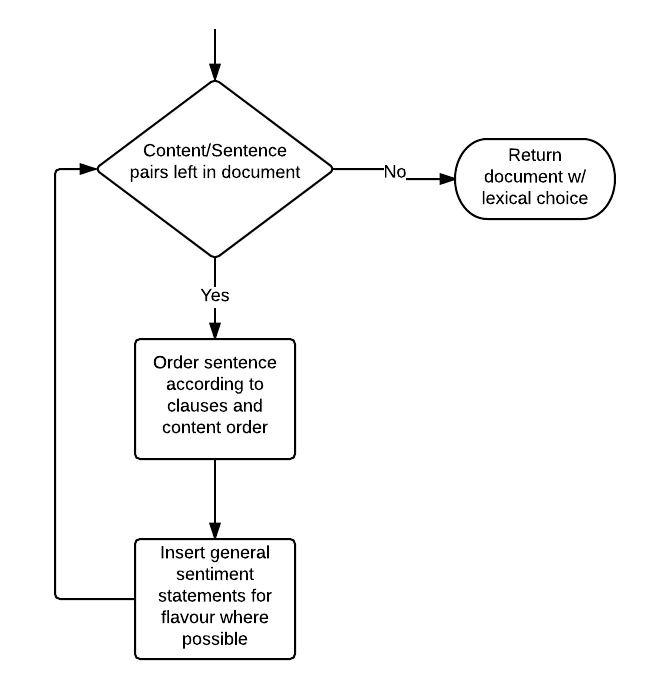
\includegraphics[width=0.7\linewidth]{figures/diagrams_etc/lex_choice}
\caption{Simple model of lexical choice, how these choices are made are heavily dependant on the type of clause.}
\label{fig:lexchoice}
\end{figure}


Referring Expressions:\\
The generation of referring expressions in NLG refers to resolving anaphora and how to refer to a particular entity within text, in order to improve the naturalness of the text created. In my case, I just needed to avoid the review sounding more robotic by referring to a person with their full name only each time, and make callbacks to their being mentioned earlier on in the text if they are. In order to resolve the issue of overuse of full name, a probability check is made and then if it passes, the full name is replaced with just the surname of the person being iterated through at this point. There is a further probability check made for repeated mentions, which includes a templated referral along the lines of 'bringing them up again'.\\



Realisation:\\
Realisation in my case essentially resolved to placing full-stops, commas and spaces in the document and converting it from a list of lists representing sentences into a single string. This was implemented mostly in a rule-based way that involved placing commas and full-stops in places that they are known to be needed in the structure of the document.\\


\section{Twitter Bot}
The Twitter bot exists in order to drive traffic towards the reviews generated and also act as a test of generating text in shorter formats than review - for example the markov chains discussed earlier are much more believable if you don't let them go on for too long. The limit of 144 characters is certainly suitable for this.\\
The bot itself uses a twitter API wrapper called Tweepy, which handles Twitter API requests required in order to make posts, search and navigate twitter.\\
The bot is programmed with two behaviours, which it enacts alternately. The first is simply the automated posting of links to movie reviews generated, with a template message that reads along the lines of "Read my review for \#filmname here". The second is to search for tweets about a movie and use that as a corpus for generating its next tweet. This aims to make the bot look like it is more realistic.\\



\section{Blog Website}
The design of the blog website is relatively simple. It is a Wordpress-like blogging website written in PHP, wish a MySQL database that stores the reviews, user information and the comments made and analytics for the site.\\
My own implementation of the website was chosen as I had prior experience making blogs in PHP, as well as the increased control over features (as I could easily modify my own code to enable/disable comments, a need for user accounts should it be targeted by spam, and analytics) seemed something which would benefit me more than the less familiar and potentially less flexible Wordpress.
I have chosen MySQL and PHP as they are languages I am familiar with, and have worked using before, as well as their being suitable for the task of a small blogging platform.\\
The website itself is a front-page which lists paginated results for movie reviews written by the movie review generator, an interface for making/creating posts, and a way to view the reviews in full. It also has user comments for gathering qualitative feedback and page visits and engagements are tracked using Google analytics and a MySQL hit-counter.\\
Along with this website, an additional site was designed to collect feedback on the reviews generated, as a back up in the event there is not enough interest in the blog. This consists of an introduction page as well as a sequential loading of text of full reviews or sentences obtained from IMdB reviews and my own generated reviews. Feedback options are whether the texts are 'human-like', 'coherent' and an additional feedback text area which users are encouraged to enter into.

